%%%%%%%%%%%%%%%%%%%%%%%%%%%%%%%%%%%%%%%%%%%%%%%%%%%%%%%%%%%%%%%%%%%%%%%%%%%%%
\chapter{Authentication and Authorization}\label{chap:authenticationandauthorization}
%%%%%%%%%%%%%%%%%%%%%%%%%%%%%%%%%%%%%%%%%%%%%%%%%%%%%%%%%%%%%%%%%%%%%%%%%%%%%

\chapterstart

“Cloud-based services, the social Web, and rapidly expanding mobile platforms will depend on identity management to provide a seamless user experience.”   (\citet{Corre:2017:WHI}).

Modern Devices are changing our everyday life. They change the way how we access information, interact with each other and share content. 
With this change of user behavior also the way we think of authentication and authorization methods has to adjust. Users find themselves struggling using multiple devices, accounts, and services. The user's burden of this site-by-site account management is putting security at risk. The goal of new authentication and authorization solutions is to help the user managing his accounts by providing single-sign-on, based on an exchange of identity-related assertion across security domains in a scalable way [cf. (\citet{Corre:2017:WHI})].  

\section{Security Considerations}

Before getting further into the topic of authentication and authorization, this section will shed light on some basic security Principles concerning authentication and authorization that help to understand the need for authentication and authorization mechanisms. 

Some basic design principles formulated by \cite{Saltzer:PICS} in 1975 were paraphrased by \cite{Neumann:2018:PTC} and are still relevant today. The principles give an underlying overview of what should be the focus when designing a secure system. The ten basic security principles are:

\begin{itemize}
	\item The economy of mechanism: Keep the design as simple as possible.
	\item Fail-safe defaults: Access should not be explicitly denied instead it should be explicitly permitted. For example when using Access Control Lists (ACLs) all access should be explicitly denied by default. 
	\item Complete mediation: Every access to every object has to be checked for authority without exceptions. 
	\item Open design: The design of an application should not be secret, it can not be assumed that design secrecy will enhance security. This principle is applied in cryptography. The design of cryptographic algorithms is available for the public, just the keys remain secret. 
	\item Separation of privileges: Two keys should be used to protect resources if feasible and privileges should be separated.  
	\item Least privilege: Every application and user should be provided with lest privileges they need to complete their job. The existence of overly powerful mechanisms such as superuser is inherently dangerous. 
	\item Least common mechanism: Minimize the amount of mechanism common to more than one user and depended on by all users.   
	\item Psychological acceptability: Keep it simple. The design of the interface for the user should be easy to understand so that the user routinely and automatically applies the protection mechanism correctly. 
	\item Work factor: Make cost-to-protect commensurate with threats and expected risks. It should not be possible to circumvent the mechanism with the resources of the attacker.   
	\item Recording of compromises: Provide trails of evidence which are tamper-proof and difficult to bypass.
\end{itemize}
	
Besides formulating these very important principles which will be discussed in various forms, \cite{Saltzer:PICS} also discus the terms "privacy" and "security". Those therms get frequently used by authors writing about information storing systems, like in this paper. However the terms "privacy" and "security" are often used very differently. \cite{Saltzer:PICS} for example, define "privacy" as the ability of an individual to specify whether, when and to whom sensible information is released. And they describe security as a technique that can control who is able to modify resources on a computer. Another more recent description of the terms "security" and "privacy" comes form \cite{Brooks:2017:IPE}. \cite{Brooks:2017:IPE} state the importance of the distinction between privacy and security. This distinction is between privacy and security are essential because there are security issues unrelated to privacy, just as there are privacy issues that are unrelated to security. While security concerns arise from illegal system behavior, privacy concerns arise from byproducts of authorized personally identifiable information (PII) processing. Even byproducts that are considered to protect PII can raise security concerns, for example, it can be questioned to which degree a tool for persistent activity monitoring should reveal information about individuals that are related to security purposes. However, security and privacy have in common that they want to protect personal information and resources or PII.

These security issues and privacy issues, of course, raise particular concerns for users as well as for companies offering authentication services. When it comes to protecting personal resources, there are three primary concerns. According to \cite{Todorov:2007:MUI} those three concerns are:  

\begin{itemize}
	\item Confidentiality: The term confidentiality means that personal information is protected from 
	disclosure to unauthorized individuals and organizations.
	\item Integrity: The integrity of information is protecting information from accidental or intentional
	tampering. Modification of confidential data may affect the data validity. 
	\item Availability: Availability is the need to be able to access information at the time a user requests it. 
The availability of the services that exposes information has to be given as well. 
\end{itemize}

In an ideal world companies offering those services will do everything to use the best technologies regarding countermeasures to protect confidentiality, integrity, and availability. Establishing countermeasures, however, can be costly leading to a trade-off between costs and level of production of information. A typical approach to establishing information security management is to analyze risks first and then form counter measurements [cf. (\cite{Todorov:2007:MUI})]. 

The result of all design principles, security and privacy considerations should be a system, network or component that is trustworthy. According to \cite{Neumann:2018:PTC} trustworthiness is given if an entity satisfies its specified requirement, after a reliable assessment. The requirements that deserve especially consideration are, those that are critical to an enterprise, mission, system, network or other entity. One of the requirements to make a system trustworthy is a reliable authentication and authorization process. These processes are discussed in more detail in the next sections.
	

\section{Authentication}

“Digital identity is the unique representation of a subject engaged in an online transaction. The process used to verify a subject’s association with their real-world identity is called identity proofing” (\citet{NIST:2017:DIG})

A digital identity as explained above is the result of what is called the authentication process. It is a way of identifying the user as whom he claims to be. For a very typical authentication process the user provides its username and password when the application demands it. If the user provides a correct username and password, an application assumes the user is indeed the owner of the account he wants to log on [cf. (\citet{Boyed:2012:GSOA})]. 

The evidence provided by the user in the authentication process is called credentials. Most of the time as mentioned above credentials get provided in the form of username and password. Nevertheless, credentials also may take other forms like PIN’s, key cards, eye scanners and so on [cf. (\citet{Todorov:2007:MUI})]. 

Credentials, which prove the identity of an entity and find use as authenticators in authentication systems, are called factors. \citet{NIST:2017:DIG} categorize following types of factors:

\begin{itemize}  
\item Something the user knows - Cognitive information the user has to remember. Examples include passwords, PIN, answers to secret questions.
\item What the user has - something the user owns. Examples include a security token, driving license, one-time password (OTP). 
What the user is - biometric information of the user. Examples include fingerprint, voice, and face.  
\item What the user is - biometric information of the user. Examples include fingerprint, voice, and face. 
\end{itemize}

 Other types of information which are not considered authentication factors but  can be used to enrich the authentication process according to \citet{Dasgupta:2017:AUA} are:
 
 \begin{itemize}
 	\item Where the user is - the location of the user can is used as a fourth factor of authentication. Examples include GPS, IP addresses.
 	\item When the user logs on - Time can also be extracted as a separate factor. Verification of employee’s identification in different office hours can prevent many kinds of grave data breaches. The time factor can easily prevent online banking fraud events to a great extent. 
 \end{itemize}

To secure a solution properly, it should at least use two factors of the three listed above. To make use of more than one factor of a pool of potential credentials to verify the identity of a user is referred to as Multi-factor Authentication (MFA). The goal of multi-factor authentication is it to provide a layered defense and make it harder for unauthorized individuals to gain access. If one of the factors breaks, the service can still rely on the non-compromised authentication factors [cf. (\citet{Dasgupta:2017:AUA})].

Using just one factor is called Single Factor Authentication(SFA). \cite{Dasgupta:2017:AUA} clearly describes the drawbacks SFA has compared to MFA, primarily the universal used password-based authentication. The user needs to remember different passwords for multiple accounts, therefore, the user often reuses one password also known as password fatigue.

In an Interview by \cite{Tomkins:2009:DPF} with Jon Brody, he explains Password Fatigue like the following. An average user has 15 accounts; some people might even have up to 30 accounts - far too much to manage appropriately. Users then tend to adopt specific password patterns like using simple passwords for nontransactional sites and complex passwords for banking sites. Since many complex passwords are hard to remember users also often reuse passwords for different services at one point - this is called password fatigue. 

Besides password fatigue \cite{Todorov:2007:MUI} draws attention to one of the significant challenges of secure user authentication represented by default passwords. Vendors often ship their devices with pre-configured standard passwords. Although vendors recommend changing default passwords, system architects and engineers often fail to do so because they are more focused on the business logic than on security causing security issues. Systems with default passwords are more straightforward to attack, for example by knowing or guessing the device the attacker has an easy time authenticating with the system accordingly. 


 Due to the problem of password fatigue and default passwords, one factor like a password might easily get compromised. The user can then no longer use the service until the repair of the system which can lead to a delay of the user when trying to access necessary information. Also, there is a risk that the user does not notice the compromise of the single factor which can lead to devastating effects [cf. (\cite{Dasgupta:2017:AUA})]. 

When designing an authentication process by using multiple factors the designers of the process should be acutely aware of the type of application and the information that has to be secured. For example, a solution for an international bank should have different standards than an app for a making a grocery list. On the one hand, challenging and complex authentication processes for trivial applications might scare away users. On the other hand, simple methods for applications protecting sensitive data might drive users away as well. Application designers should always try to find a middle way that suits both parties, the application owners and the users [cf. (\cite{NIST:2017:DIG})]. 

The factors are an important part of the authentication process which result should be an authenticated user. However, to become an authenticated user the user has to go through certain steps on the way. These steps the user has to go through are enabled be typical components unique to the authentication process. \cite{Todorov:2007:MUI} identifies three typical components that are part of the authentication:

 \begin{itemize}
 \item The Supplicant is the party that provides the evidence to prove the identity of a user or client. The result of the authentication process should be the authenticated user or client.  
 \item The Authenticator, also called server, is responsible for ascertaining the user identity. After prove of identity, the authenticator can authorize or audit the user access to resources. 
 \item Security Authority Database, which is storage or  a mechanism to check the user's credentials. The storage can be represented by as much as a flat file, a server on the network providing centralized user authentication or a distributed authentication server. 
\end{itemize}

\begin{figure}[h]
	\centering
	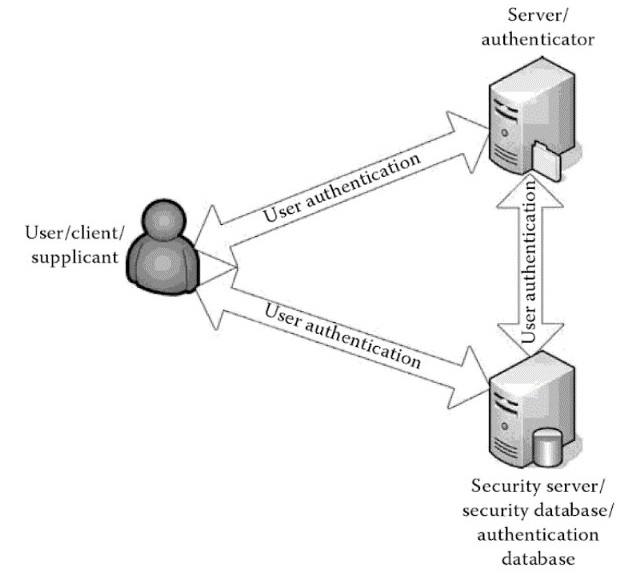
\includegraphics[width=0.8\textwidth]{images/componentsUserAuthenticationSystem}
	\caption[Componets Authentication]{Components User Authentication System}
	\label{fig:componentsuserauthenticationsystem}
\end{figure}


It is vital that all the components like shown in (figure~\ref{fig:componentsuserauthenticationsystem}), of a user authentication system can communicate independently of each other. Whether or not all communication channels are used depends on the authentication mechanism and the model of trust that it implements. For example, the Kerberos authentication protocol does not feature direct communication between the authenticator and security server [cf. (\cite{Todorov:2007:MUI})]. 

Application security is a complex task and developing a customized siloed identity solution can be expensive. A Stand-alone identity store can besides being expensive also causes information assurance and administrative problems for organizations  [cf.(\cite{JerichoSystems:IS})]. 

  A federate authentication or identity federation says \cite{Boyed:2012:GSOA} is a system that is maintaining its accounts, for example, username and password databases, with the help of third party service. Often big cooperate IT environments already use such solutions. Environment applications, for example, may trust an Active Directory server, an LDAP server or a SAML provider.    \cite{NIST:2017:DIG} also claims that identity federation is preferred over some siloed identity solution that each serve a single agency or Relying Party (RPs). Furthermore \cite{NIST:2017:DIG} lists certain benefits that come with using federated architectures, as can be examined before. 

\begin{itemize}
\item Enhanced user experience. For example, an individual can be identity proofed once and reuse the issued credential at multiple RPs. 
\item Cost reduction to both the user (reduction in authenticators) and the agency (reduction in information technology infrastructure). 
\item Data minimization as agencies does not need to pay for collection, storage, disposal, and compliance activities related to storing personal information. 
\item Pseudonymous attribute assertions as agencies can request a minimized set of attributes, to include claims, to fulfill service delivery. 
\item Mission enablement as agencies can focus on the mission, rather than the business of identity management.
\end{itemize}

To reflect on authentication it can be said that authentication is a very important part of every applications. As users are getting more concerned on security the pressure on developers grows to provide a solution that secures sensible data while keeping up usability standards, which can often be a trade-off. Complex applications need complex security which can mean high costs for individually developed solutions; therefore application developers should also think about using federate authentication solutions. 


\section{Authorization}


The authentication and authorization process are very closely related to each other and for users often hard to separate. After the authentication process of a user, the application has now proof that the user is who he claims to be, but not every user is the same. After  the user authenticates, the user may want to access data or services. Based on the information provided by the authentication process the application has the possibility to allow or deny the user to access information or services. In other words we have to check if the user is authorized to access data of a service. Furthermore authorization, offers granular control to distinguish between read, write or execute access to individual resources, typically access control list (ACL) are used for each operation [cf.(\cite{Todorov:2007:MUI}, \cite{Boyed:2012:GSOA})].

  Systems offer a user login process or sign-in process, in order to receive the information necessary to make authorization decisions. The login process initiates the authentication process between user and the system. As a result of this process, the user receives a system or application specific structure called an access token. The access token holds information about the user which will indicate what kind of resources the user can access. For every action the user then has to provide the access token and based on the information provided within the access token is then either granted or denied access [cf. (\cite{Todorov:2007:MUI})]. 

Delegated authorization is granting access to another person or application to act on behalf of the user.
\cite{Boyed:2012:GSOA}


\section{Token-base Authentication}


The way web developers write back-end applications has changed significantly with the rising popularity of single page and mobile applications. Backend-developers no longer spend a lot of time building markup. Instead, they build APIs for front-end applications to consume. The split up of front-end and back-end allows the back-end to focus on business logic and data management while the front-end solely focus on the representation of the content. The number one way single page and mobile web applications are authenticating users according to \cite{Tkalec:2015} is token-based authentication.

\cite{Serilleja:2015:Scothio} shares the view that token-based authentication is the modern way to handle authentication. Token-based authentication should be considered because of various factors. It is optimal for mobile applications which work in a stateless way and need to adapt to the sudden change of demand in a scalable way. Furthermore, token-based authentication provides extra security and applications can pass on authenticated users to other applications. However before taking a closer look at token-based authentication, it should be taken into account how \cite{Serilleja:2015:Scothio} and \cite{Tkalec:2015} concluded that token-based authentication is the best alternative for modern web applications to authenticate their users. Therefore, \cite{Serilleja:2015:Scothio} for example examines how authentication was done in the past. One approach to authenticate users used in th past that puts token-based authentication in perspective is server-based authentication. 

\paragraph{Server-Based Authentication.}
A lot of modern-day API’s built on the Representational State Transfer(REST) programming paradigm which basis is the HTTP protocol which is stateless as well. A protocol that is stateless does not recall the actions that were taken beforehand which means for example that if we authenticate the user, in the next request we have to authenticate the user again because the application will not know the user anymore [cf. (\cite{Serilleja:2015:Scothio})]. 

The aim of server-based authentication is for the application to remember the user that logged on at the application. The application has to store the information on the server, which can be done in a few different ways on the session, usually in memory on the disk. The workflow of a server-based authentication starts with the server delivering the website and the user logging in with username and password. The server saves the information from the user login info in a session. After the session is established, the session is checked on the server for every request. If the session is valid, the server returns the requested data to the server. However, since modern single-application ant mobile applications are on the rise, this method to authenticate user shown some problems, especially when it comes to scalability [cf. (\cite{Serilleja:2015:Scothio})]. 

The session handling with server-based authentication is especially hard on the server’s bandwidth. Most of the time the session gets established in memory on the server when the user authenticates. This approach leads to an enormous overhead. The second problem with this approach is that the information of the user is held in memory on the server. Since more and more companies are moving servers to the cloud, this is not only a security issue but replicating servers to scale is limited. Also nowadays users want to access their data at any moment from every device. Providing the user with the possibility to access data across multiple mobile devices is vital, which means cross-origin resource sharing has to be enabled. With server-based authentication, it is possible to run into problems with the forbidden request when the user tries to access data from another domain [cf. (\cite{Serilleja:2015:Scothio})].


\paragraph{
	Token-based authentication with JSON Web Token
}

The most important thing about token-based authentication is that it is stateless, much like HTTP. The server does not have to hold the session of the user over an extended period on the server. Instead, the user can request resources by offering a token generated by an authentication server. The token send in the query string or Authorization header can then be validated at the resource server, and the secure resource will be returned to the user. The approach of using JSON Web Tokens gives one the ability to scale applications without considering on which domain the user logged on. Another advantage besides being scalable is that token-based authentication gives one the possibility to reuse the same token for authenticating the user. Therefore, it gets easier to build applications that share permission with other application because many separate servers, running on multiple platforms and domains can reuse the same token. The approach also gives performance advantages compared to server-side authentication because there is no need to find and deserialize the session on each request. However, since it is best practice to encrypt the token, the token still needs to be validated, and the content needs to be parsed. One way to implement token-based authentication is with the help of JSON Web Tokens. JSON Web Tokens are gaining popularity fast and are backed by huge companies like Google and Microsoft. Also the Internet Engineering Task Force defines a standard specification. OpenID and OAuth also use the JSON Web Token as a standard; therefore, the usage of the JSON Web Token will be explained in detail [cf. (\cite{Tkalec:2015})].


JSON Web Token (JWT) is a compact structure that holds information about the authentication of a user or claims. The structure is indented for space-constrained environments such as HTTP Authorization headers. The payload of the JSON Web Token is of JSON, enabling the claims to be digitally signed or integrity protected with a Message Authentication Code (MAC) and encrypted [cf. (\cite{JWT:IETF:Jones:2015})].

The standard is used to transport data between interested parties. The transferred data can be for example the identity of a user or user’s entitlements. Furthermore, with the possibility of digital signatures and encryption data can be transferred securely over an unsecured channel. The signatures also allow asserting the identity of a user if the recipient trusts JWT asserting party [cf. (\cite{Siriwardena:JWTJWSJWE:2016})].

An example of a JWT Token is an id\_token. Google provides for Developers an OAuth 2.0 Playground, where developers can choose a scope and try it out against the Google API. To get an excellent example of a JWT, I selected the OAuth2 API v2 and authorized the API [cf. (\cite{Google:2018:OAuthPlayground})].


\begin{figure}[h]
	\centering
	
\includegraphics[width=0.8\linewidth]{images/googleOAuthPlaygroundOAuthAPI}
	\caption[OAuth API]{Google Developers Playground OAuth 2.0 API}
	\label{fig:googleoauthplaygroundoauthapi}
\end{figure}

After choosing and authorizing, the API Google returns an Authorization Code. This Authorization Code is specific for a certain Authentication Flow defined by OAuth and can then be exchanged for the tokens. As a result all information for the scopes that where selected beforehand is returned. Because OAuth 2 API v2 was selected, the returned value is an id\_token. This id\_token is a nice representation of a JWT and holds the standard information that are required according to the OAuth specification  [cf. (\cite{Google:2018:OAuthPlayground})].


\lstset{caption=JWT Token,breaklines=true, breakatwhitespace=true, basicstyle=\small\ttfamily, label=lst:jwt, tabsize=3, basewidth={0.55em}, fontadjust, language=XML}

\begin{lstlisting}
eyJhbGciOiJSUzI1NiIsImtpZCI6ImRhZDQ0NzM5NTc2NDg1ZWMzMGQyMjg4NDJlNzNh
Y2UwYmMzNjdiYzQifQ
.
eyJhenAiOiI0MDc0MDg3MTgxOTIuYXBwcy5nb29nbGV1c2VyY29udGVudC5jb20iLCJh
dWQiOiI0MDc0MDg3MTgxOTIuYXBwcy5nb29nbGV1c2VyY29udGVudC5jb20iLCJzdWIi
OiIxMTIzMDE5MzgzMjI4MTAyMzk3MTIiLCJlbWFpbCI6ImNvcm5lbGlhcmF1Y2hAZ214
LmF0IiwiZW1haWxfdmVyaWZpZWQiOnRydWUsImF0X2hhc2giOiJSdjJRQjZoZzFqdDZR
aHRJWG5laWVnIiwiZXhwIjoxNTI5NzQ3MTk2LCJpc3MiOiJodHRwczovL2FjY291bnRz
Lmdvb2dsZS5jb20iLCJpYXQiOjE1Mjk3NDM1OTYsIm5hbWUiOiJDb25ueSBSYXVjaCIs
InBpY3R1cmUiOiJodHRwczovL2xoNC5nb29nbGV1c2VyY29udGVudC5jb20vLWJFbEt3
aDVaNUJnL0FBQUFBQUFBQUFJL0FBQUFBQUFBQk5rL0p5Qm1XTW9uYUlJL3M5Ni1jL3Bo
b3RvLmpwZyIsImdpdmVuX25hbWUiOiJDb25ueSIsImZhbWlseV9uYW1lIjoiUmF1Y2gi
LCJsb2NhbGUiOiJkZSJ9
.
yibOtrXy9_-cfOWytzwGuE4zqLv-MK_2-PYIKR_xecJt9ACnMnNMSmio6i8Vu7U061wF
OTb-qRennHbvy3lTRZLcTXttIrIUl-NdnZs2BrTSGWrw9aRzEjIHAXiY4fGRHj9VZXs_
_J3Nn0EoBmT7Cnua2hb4U_X3hAyGpEvlSGKc5HvbyzOAtNh081Cyj1TI-AidCPTuC5vh
68C55tLJ87PWNm8WU1rCPOPBdVTjhYlqJKCpgUJ39_p_MXL_uHBZXRrvbOyV_tZVlw47
rjd8GFnBq1QqsYAR-6wrFbNL1pY6tPyriqZnQdi5KqYWPUwGpXbFDUfhZAmWXT8-PTsc
gQETEp8o3RvRHtfSu8Gx4UOhukt9_VxVdHmpFw
\end{lstlisting}


The JWT Token in the figure above is presented as a sequence of URL-save base64url-encoded values. The different values are separated by a (‘.’) character. How many parts a JWT has is dependent on how the JWT is serialized. Either by using the JWS Compact Serialization or JWE Compact Serialization  [cf. (\cite{JWT:IETF:Jones:2015})].


To make sense of this JWT token in the figure above it is best to look at each of the three parts of the JWT separately. When decoding the first part of the JWT we receive a JSON object. Each part can be decoded individually but if a quick representation of a token is needed developers are best advice to use \href{https://jwt.io/} {https://jwt.io/}. The website not only decodes the information of the token it also verifies the token.The figure above shows a warning that pops up if the token is not flawless. The verification of the token and the signing is done with multiple libraries that inform about certain vulnerabilities of the JSON Web Token. The first decoded part of the JWT gives us the following JSON.


\lstset{
	caption=JOSE Header,
	label=lst:joseheader
	string=[s]{"}{"},
	stringstyle=\color{blue},
	comment=[l]{:},
	commentstyle=\color{black}
}
\begin{lstlisting}
{
	"alg": "HS256",
	"typ": "JWT"
}
\end{lstlisting}


This is the JOSE Header, representing the type of the token, the cryptographic operation applied and optionally additional properties of the JWT. Based on the information of the JOSE Header it can be said if the JWT is a JWS or a JWE. When speaking of JWT we speak of one of the implementations of JWT because in fact JWT does not exist itself. Concrete implementation of the JWT are JSON Web Signature (JWS) or JSON Web (Encryption). The figure below gives an optical representation of the structure [cf. (\cite{Siriwardena:JWTJWSJWE:2016})].


\begin{figure}[h]
	\centering
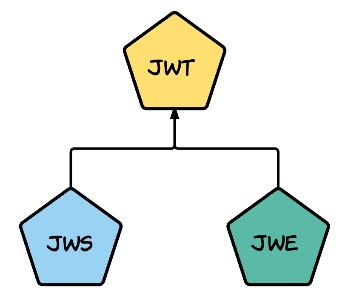
\includegraphics[width=0.8\linewidth]{images/jwtjwsjwe}
\caption[JWT Inheritence]{JWT Inheritance}
\label{fig:jwtjwsjwe}
\end{figure}



\section{Single Sign-On}

The aim of Single Sign-On(SSO) is to design an authentication system that serves the interests of the user as well as the interests of the service provider. Whereas the user prefers a simple process, the service provider requires a complicated authentication procedure. Ironically trying to make the authentication procedure more save often leads to weakening the whole system due to the user always  finding new ways to bypass it. An example mentioned before is password fatigue. Another challenge that SSO is trying to tackle is that standard web authentication solutions that require the user to login with a password, only authenticate the user and are not capable of providing access control or revealing additional information about the user. Most SSO solutions try to combine the authentication process and authorization [cf. (\cite{Prochazka:2010:UCA})].

According to \cite{Lynch:2017:IIG} two SSO solutions gained broad acceptance. On the one hand, SAML-based federations using SOAP, focusing on large enterprises also including governments and educational networks. On the other hand, the Web Authorization Protocol was introduced which is a combination of the Protocols OpenID and OAuth. SAML federations have been customized to address the security concerns of those institutions that typically have a large user base, significantly protected resources, complex authorization patterns and data and services spread across multiple domains. However, in a Web 2.0 world, the SAML solutions where seen as too rigid and too severe to maintain; a lightweight SSO was needed, therefore the Web Authorization Protocol was designed. The approach of this protocol is taking advantage of the lightweight RESTful APIs which are reusing the existing HTTP architecture features and the JavaScript Object Notation(JSON).

One of the well-known solutions based on Security Assertion Markup Language version 2 (SAML2) is Shibboleth. Shibboleth is one of the leading middlewares for building identity federations in a higher education sphere. To offer authentication, authorization and attribute assertion between entities. \cite{Prochazka:2010:UCA} identifies following entities defined by Shibboleth are:

\begin{itemize}
	\item Identity Provider (IdP)
	\item Service Provider (SP)
	\item Discovery Service
	\item Metadata Operator
	\item Federation Operator
\end{itemize}

 The discovery service is used to find the users organization IdP. The IdP defines an attribute release policy and releases different sets of the user's attributes to different SPs. Users are only able to agree or disagree with the whole set of attributes because the decision comes from the IdP. When the user tries to log on, to a service of a Service Provider, he gets redirected to a page where he can choose and IdP previously found by the Discovery Service. If an SP wants to provide its service to multiple federations it has to negotiate policy and technical detail with each federation operator. The federation operator manages the federation policies and introduces SPs and IdPs. Furthermore, the federations operator has to maintain and manage the information about all entities in a federation which is contained in the Metadata. A problem with this architecture is that the SP has to keep track of changes of the technical specification of various federation operators to maintain the configuration for each federation operator. A solution would be a significant federation registration, but this is indeed not possible because of technical and administrative severity and political will. This solution is also somewhat misleading for users since they have to maintain multiple credentials, select from multiple identifiers and so on [cf.\cite{Prochazka:2010:UCA}].
 
 According to \cite{Prochazka:2010:UCA} Shibboleth is too restrictive, a solution with a centrally managed point of IdPs and SPs is preferred. Also, users should not have to deal with redundant accounts.





\chapterend